\chapter{Team 6 Agent Design}\label{team_6_agent_design}

\section{Introduction}

Our agent has been designed to maximise both individual and collective ability. This has been achieved by maintaining four core beliefs:

\begin{itemize}
    \item Greed should be punished
    \item Irrationality should be punished
    \item Maintaining a team of semi-greedy, semi-rational agents is best for the collective
    \item Collective Intelligence and Group Think should be used under the right conditions
\end{itemize}
With these beliefs in mind, an overall strategy was devised:
\begin{itemize}
    \item Use a Social Capital system as the main driver for agent decision making
    \item Define a robust set of objectives for the Social Capital system
    \item Integrate learning into the system
\end{itemize}

\section{Social Capital System}

The main driver behind our agent's decision making is the Social Capital system. The system was designed with two key objectives in mind - effectively managing finite common pool resources (avoiding the tragedy of the commons), and maximising self and collective utility. When combined, these improve the chance of escaping the pit. The system is also subject to three constraints - maximising agent state, obtaining a favourable loot distribution, and electing the most favourable leader.\\

To meet the requirements set out, five values are maintained for each agent in the game. The values are continuously updated as the game evolves. The values are:

\begin{itemize}
    \item Generosity (G)
    \item Bravery (B)
    \item Similarity (S)
    \item Leadership (L)
    \item Trust (T)
\end{itemize}

Each measure takes a value in the range [0,100] and is initialised to 50, with the exception of Bravery which is initialised to 100.

\subsection{Generosity}

The generosity value is used to track how generous an agent is when we trade with them. For example, another agent gifting us an item would be seen as generous, particularly if the item gifted is of higher value than our own. The value is updated as per (\ref{eq:T6GenerosityFormula}).

\begin{equation}\label{eq:T6GenerosityFormula}
    G_{i} = G_{i} + (O_{v} - D_{v})
\end{equation}
Where $G_{i}$ is the Generosity of the $i$th agent, $O_{v}$ is the value of the item being offered, and $D_{v}$ is the minimum value of the item being demanded.

\subsection{Bravery}

The Bravery value is used to track how often an agent either attacks or defends. The value itself is the proportion of rounds in which an agent fought or defended, rounded to the nearest integer. A value of 100 indicates that an agent never cowers, whereas a value of 0 indicates that an agent always cowers. This value aligns with the core belief that greed should be punished - not fighting is a form of greed, therefore an agent that doesn't fight is penalised.\\

The value is updated at the end of each level. Note that each level can consist of multiple fight rounds, therefore an agent's bravery value can change significantly.

\subsection{Similarity}

The Similarity value is used to track how closely another agents beliefs align with our own. This is achieved by comparing proposals (both loot and fight) with our own. It is believed that an agent's overall beliefs and strategy are well represented by their proposals, which makes this an attractive method for updating the value.\\

Whenever a proposal is received, either to vote on, or to be shared by us when we are the leader, (\ref{eq:T6SimilarityFormula}) is used to update the Similarity value for the proposer.

\begin{equation}\label{eq:T6SimilarityFormula}
    \begin{aligned}
    S_{i}=S_{i}+10(Sim(P_{i})-0.5) \\
    Sim(P) = \frac{1}{n}\sum_{k=1}^{n}f(P(A_{k}),P_{u}(A_{k})) \\
    f(D_{1},D_{2})=\left\{
    	\begin{array}{ll}
    		1 & \mbox{, if } D_{1} = D_{2} \\
    		0 & \mbox{, otherwise} 
    	\end{array}\right.
    \end{aligned}
\end{equation}
Where $S_{i}$ is the Similarity agent for the $i$th agent (the proposer), $P_{i}$ is the received proposal, $P_{u}$ is our own proposal, and $A_{1..n}$ is an array of predetermined agent states. The basic idea is to test both our own proposal and the received proposal on a range of agent states, and calculate the proportion of decisions (based on the agent states) that are equivalent when both proposals are applied. This gives a value in the range [0,1].

\subsection{Leadership}

There are three main factors that are considered when updating the Leadership value:

\begin{itemize}
    \item Freedom of Information - the leader should share proposals with the collective
    \item Change in agent state - the purpose of the leader is to improve the collective's success chances, therefore it is appropriate to judge the leader by the overall state of agents
    \item Responsibility - an agent shouldn't cower just because they are the leader, they should lead by example
\end{itemize}

Counts are maintained for the total number of proposals received, and the number of proposals received in the current round. At the end of each round, the leadership value is updated based on a comparison between the average number of proposals received per round, versus the number of proposals received in the current round. The relevant update is outlined by (\ref{eq:T6LeadershipFOIFormula}).

\begin{equation}\label{eq:T6LeadershipFOIFormula}
    L_{L} = L_{L} + \frac{P_{c}-P_{a}}{4}
\end{equation}
Where $P_{c}$ is the number of proposals received in the current round, and $P_{a}$ is the average number of proposals received per round.\\

The final update occurs whenever a new leader is elected. The agent stores the Bravery value for the leader at the time of their appointment. At the end of their term, their current Bravery value is compared to the value at the start of their term. As the leader is expected to lead by example, any reduction in Bravery is punished, and any increase is rewarded. (\ref{eq:T6LeadershipBravery}) outlines the process.

\begin{equation}\label{eq:T6LeadershipBravery}
    L_{L} = L_{L} + Max(-5,Min((B_{L}^{t}-B_{L}^{t-}),5))
\end{equation}
Where $B_{L}^{t-}$ is the leader's Bravery at the start of their term, and $B_{L}^{t}$ is the corresponding value at the end of their term.

\subsection{Trust}

The Trust value is a measure of how dependable other agents are. If an agent is told to take a certain action by the leader, do they comply or defect? At the end of each level a list of defectors is published by the game. All agents on this list have their Trust value decreased as per (\ref{eq:T6TrustFormula}). Complying agents have their value increased.

\begin{equation}\label{eq:T6TrustFormula}
    T_{i}=\left\{
    	\begin{array}{ll}
    		T_{i}-10 & \mbox{, if agent i is on defector list} \\
    		T_{i}+2  & \mbox{, otherwise} 
    	\end{array}\right.
\end{equation}
Where $T_{i}$ is the Trust value for the $i$th agent.\\

If an agent defects, it takes 5 rounds of compliance to recover its initial trust value. This allows our agent to forgive those agents that only occasionally defect. Serial offenders will clearly be severely punished.

\section{Fighting}

\subsection{Fight Decisions}

The agent has its own internal rules for when it should attack, defend, and cower. These rules are based on the agent's state relative to its initial state. For example, if HP, Stamina, and Attack are all above the relevant thresholds, our agent will choose to attack. In the instances where the agent isn't given a proposed action, it will follow its own internal rules. If the agent is told what course of action to take, it follows this unless the internal rules tell it to cower and the proposal doesn't, in which case the agent will defect and cower. It is believed that the agent is in the best position to decide whether or not it should cower, as it has the best visibility of its own state.

\subsection{Fight Proposals}\label{T6FightProposals}

Our agent generates a fight proposal each round. This includes a number of rules based on an agent's state, and the fight action that should be taken if the condition is met. This proposal is sent to the leader 10\% of the time. Proposals received are compared to our own proposal, using the $Sim$ function from (\ref{eq:T6SimilarityFormula}). If the similarity score is $\geq 0.8$, the agent votes \textbf{for} the proposal, else the agent votes \textbf{against} the proposal.

\section{Loot}

\subsection{Loot Distribution Decisions}

Our agent has its own idea of what loot it requires based on its current state. However, loot distribution is a difficult task, and defecting can result in not getting any loot at all. Therefore, our agent takes the loot proposed to it. If there is no proposal, our agent randomly chooses a piece of loot that is most beneficial - if health is the lowest value relative to its starting value, the agent will randomly choose a health potion. This helps to increase the chance of the agent receiving the loot, as purely rational agents would always go for the best loot possible.

\subsection{Loot Proposals}

All logic here is almost identical to \ref{T6FightProposals}. Only an agent's `needs' can be used to decide the loot distribution with the current proposal implementation. Therefore our agent generates its own proposal, sends it to the leader 10\% of the time, and uses similarity when voting on received proposals.

\subsection{Trading}

Trading is an essential part of the game, and if used properly can be very beneficial to the collective. Our trading strategy strikes a balance between selfishness and selflessness, so as to maximise both individual and collective utility. Each agent can be involved in multiple trade negotiations at once.
If our agent is not currently involved in a trade negotiation:

\begin{itemize}
    \item Determine if we want a weapon or shield (whichever is currently lower)
    \item Find an agent with a better version of that item (can iterate over agent states)
    \item Open a trade negotiation with that agent, offering the best item we wouldn't be using after the trade
\end{itemize}
When our agent receives incoming trade requests:

\begin{itemize}
    \item Accept any gifts (we can use these in later trades even if we don't use the weapon/shield)
    \item Decline any trades we can't partake in (don't have an item to satisfy the other agent)
    \item Accept if the agent is worse off than us and we can help without hindering ourselves (e.g. if they want a shield and our second best shield is better than their best shield, offer our second best shield)
    \item Accept if after the trade the sum of our Bonus Attack and Bonus Defense is greater than it was before the trade
    \item Accept if we really like the other agent (weighted sum of Social Capital values $\geq 0.8$)
    \item Decline in all other instances
\end{itemize}

This strategy allows us to improve our individual utility, increase other's utility without affecting our own, and to help agents we hold in high regard in times of need. This balanced approach ensures all agents should have access to the highest rated weapons and shields if they need them, and also allows us to prevent bad actors from hoarding items.

\section{Leadership}

\subsection{Running for Leader}\label{T6RunningForLeader}

Currently the game requires all agents to submit a leadership manifesto whenever a new leader needs to be appointed. Our agent has an initial idea of what a good manifesto looks like (`good' in this sense means both advantageous to the collective, and also likely to be viewed favourably by other agents). This initial manifesto is:

\begin{itemize}
    \item Not holding the loot decision power
    \item Not holding the fight decision power
    \item Term length of 3 levels
    \item Overthrow threshold of 51\% for no confidence votes
\end{itemize}

Our agent appreciates that its initial guess might not be great, so the manifesto dynamically changes as the game progresses. This is to both increase the likelihood of being selected, and for the benefit of the collective. The agent maintains an opinion for both the loot and fight decision powers. These opinions are in the range [0,100], where $>50$ means \textbf{should} have the power, and $\leq 50$ means \textbf{should not} have the power. Both values are initialised to 25, indicating that the agent believes it shouldn't hold either power as leader.\\

Values are also stored for term length and overthrow threshold. These are both floating point numbers to allow for fine tuning. All values are updated as per (\ref{eq:T6ManifestoFormula}), and then restricted to an appropriate range (e.g. [1,10] for term length).

\begin{equation}\label{eq:T6ManifestoFormula}
    V_{u} = V_{u} + (L_{i}-50)*(V_{L}-V_{u}/100)
\end{equation}
Where $V_{u}$ is our agents value for a given manifesto element, $V_{L}$ is the value the previous leader was elected with (in the case of power values, this takes value 0 or 100), and $L_{i}$ is the outgoing leader's Leadership value. The same update is performed to all four elements of the election manifesto.\\

Manifesto creation involves updating the manifesto values, converting the power values to concrete decisions, and sending the manifesto to be voted on.

\subsection{Fight Decisions}

Our initial manifesto does not give our agent the power to overrule fight decisions. However, that manifesto can change, as outlined in \ref{T6RunningForLeader}, such that it is possible for our agent to be elected with the power to overrule fight decisions. One of our agent's beliefs is that freedom of information is to the advantage of the collective. Therefore, a reasonable proportions of fight proposals received as leader should be made available to all other agents. Once again, proposal similarity is used in this decision making. A similarity score is generated by the `Sim' function in (\ref{eq:T6SimilarityFormula}), and if this value is $>0.6$ then the proposal is shared. This allows us as leader to influence the fight without appearing dictatorial. Once a proposal has been voted for, the proposed actions are sent to each agent unchanged, respecting the democratic outcome. Any agents that don't agree with the proposed action always have the opportunity to defect.

\subsection{Loot Decisions}

Logic for loot decisions is much the same as it was for fight decisions. This includes broadcasting any proposals that are more than 60\% similar to our own. One significant difference is inspired by Rescher, who introduces the concept of the `canons of distributive justice', which are derived from seven ways of treating people:

\begin{enumerate}
    \item ``as equals
    \item according to their needs
    \item according to their ability or merit or achievements
    \item according to their efforts and sacrifices
    \item according to their actual productive contribution
    \item according to the requirements of the common good, or the public interest, or the welfare of mankind, or the greater good of a greater number
    \item according to a valuation of their socially useful services in terms of supply and demand" \cite{rescher1966}
\end{enumerate}

The canons are to be considered in a given context, and `legitimate claims' established. In the context of the game and our Social Capital system, four canons were identified as related to `legitimate claims':

\begin{enumerate}
    \item The canon of Need
    \item The canon of Productivity
    \item The canon of Social Utility
    \item The canon of Supply and Demand
\end{enumerate}

As leader, our agent looks at the loot allocation according to the proposal chosen by other agents. In cases where multiple agents are vying for the same piece of loot based solely on their needs, the other three canons are taken into consideration. The concepts of Productivity and Social Utility are not the easiest to quantify, particularly as it is hard to know the impact one single agent has had on the outcome of a fight. However, these canons can be considered in the context of the Social Capital values. Therefore, separating agent's loot requests can be resolved by using a weighted average of all Social Capital values. They are all relevant to the canons, e.g. high bravery indicates a productive contribution to society and fighting even when other agents cower.

\section{Elections}

\subsection{Leadership Elections}

Votes in leadership elections are critical for two main reasons:
\begin{enumerate}
    \item The leader can wield significant power
    \item Very few votes are required for a leader to be elected
\end{enumerate}
It is therefore of the utmost importance that our agent votes for a `good' leader. The following algorithm is used to vote:
\begin{enumerate}
    \item Generate a manifesto score
    \item Generate an opinion of the agent (weighted average of Social Capital values)
    \item Overall score = manifesto score * opinion
    \item Rank candidates according to overall score
    \item Vote for the highest ranked candidate (in case of plurality vote)
\end{enumerate}
The manifesto score is a value in the range [0,1], where 1 indicates that the manifesto is identical to our own. The score tends to 0 as a manifesto increasingly deviates from our own. The score is calculated according to (\ref{eq:T6ManifestoScore}).

\begin{equation}\label{eq:T6ManifestoScore}
    M_{i}=\left\{
    	\begin{array}{ll}
    		0 & \mbox{, if } TL > 10 \mbox{ or } OT > 75 \\
    	  \sum_{k=1}^{4}\frac{1}{4+\left | U_{k} - C_{k} \right |} & \mbox{, otherwise} 
    	\end{array}\right.
\end{equation}
Where $TL$ is the manifesto's term length, $OT$ is the manifesto's overthrow threshold, $U_k$ is our value for 
the $k$th manifesto element, and $C_k$ is the corresponding value from the candidate's manifesto.\\

(\ref{eq:T6LeadershipOpinion}) is used to calculate the opinion score.

\begin{equation}\label{eq:T6LeadershipOpinion}
    O_{i}=\left\{
    	\begin{array}{ll}
    		0 & \mbox{, if } L_{i} < 40 \\
    	  0.5 * L_{i} + 0.2 * S_{i} + 0.15 * T_{i} + 0.1 * B_{i} + 0.05 * G_{i} & \mbox{, otherwise} 
    	\end{array}\right.
\end{equation}
Where all variables are the social capital values for the $i$th agent (the candidate).\\

Once both scores have been calculated, the overall score can be derived (\ref{eq:T6OverallLeadershipFormula}).

\begin{equation}\label{eq:T6OverallLeadershipFormula}
    R_{i} = M_{i} * O_{i}
\end{equation}

All candidates are ranked based on their score $R_{i}$, and in the case of plurality voting the top ranked candidate is chosen. If Borda count is used, all agents with a score $\geq 0.5$ are put on the ballot. If no agents meet this threshold, the agent votes for itself.

\subsection{No Confidence Votes}

For no-confidence votes, a combination of Social Capital values and objective success are used to determine our vote. In this instance objective success refers to the number of agents that died in the most recent round.\\

Much like in leadership elections, an overall opinion of the leader is derived from their social capital values, as per (\ref{eq:T6NoConfidenceOpinionFormula}). This is then multiplied by a scaling factor, giving a final measure of the leader's performance (\ref{eq:T6AgentDeathsFormula}, \ref{eq:T6NoConfidenceValue}).

\begin{equation}\label{eq:T6NoConfidenceOpinionFormula}
    O_{L} = 0.5 * L_{L} + 0.2 * S_{L} + 0.15 * T_{L} + 0.1 * B_{L} + 0.05 * G_{L}
\end{equation}

\begin{equation}\label{eq:T6AgentDeathsFormula}
    \delta = \frac{1}{1+0.25*AD}
\end{equation}
Where $AD$ is the number of agent deaths in the most recent round.

\begin{equation}\label{eq:T6NoConfidenceValue}
    N_{L} = \delta * O_{L} 
\end{equation}
If $N_{L} > 55$ vote `positive', else if $N_L < 45$ vote `negative', else `abstain' as the agent has no strong opinion either way.

\section{HP Pool Donation}

The HP Pool donation mechanic is a powerful one - it allows agents to skip a level without fighting. At the same time, agents must be careful not to give away too much health, as they then won't be able to fight. Our agent donates a proportion of its health where possible (up to a maximum of 10\% of the starting health in any given round). Before a fight, the agent approximates what its state will be after the fight. It then donates as much health as possible (up to the limit), taking into consideration the health needed going into the fight to almost guarantee survival.

\section{Collective Intelligence and Group think}
\subsection{Collective Intelligence (CI)}
In so far, most decision-making will be shaped by each agent's individual beliefs and the social capital system. However, in such a diverse collective community, it is important to note that knowledge is distributed amongst all agents. As such, even though each agent may believe they are making the most rational decision, this is based on the fact that, in most cases, the decision being made is informed by the information and knowledge available to the agent at the time when the decision was made.\\

However, should this agent access the information and knowledge held by other agents, it is likely that they may be able to make more rational decisions, hence maximizing their utility, within their self-defined social capital values.\\

Representative of our society, this game has introduced the concept of distributed knowledge by adding a level of anonymity to each agent state, such as the health of each agent being only accessible in discrete levels, or not being able to access information regarding other agents' inventory.\\

This introduces the idea of collective intelligence, where given that knowledge is distributed, the  individuals should share their knowledge, data, and skills such that through collaboration and communication, it should be possible to maximize collective utility.

\subsubsection{Communication}
In many cases, it may not be possible to communicate this distributed knowledge effectively. In such a time and resource-limited environment facing imminent danger, the cost of this communication could be too high. In other cases, it may not even be possible. Alternatively, some agents may choose to not participate in any collaboration or communication.  What system can be used which can capitalise on collective intelligence with minimal communication, dispute resolution, and computational cost? \\ 

There must be a way in which each agent should implicitly be able to observe other agents and make informed decisions, on whether an agent may have some information, not available to them, which they can use to maximize their self-utility.

\subsection{Groupthink (GT)}
This behaviour can be observed in nature. Consider figure \ref{fig:T6Fish} showing a shoal of fish. \\

\begin{figure}[h]           %this opens a floating environment. It will move around. The [h] tells the compiler to put the image [h]ere, not at the [t]op, [b]ottom or on a separate [p]age
	\centering				%put the figure in the middle of the page
	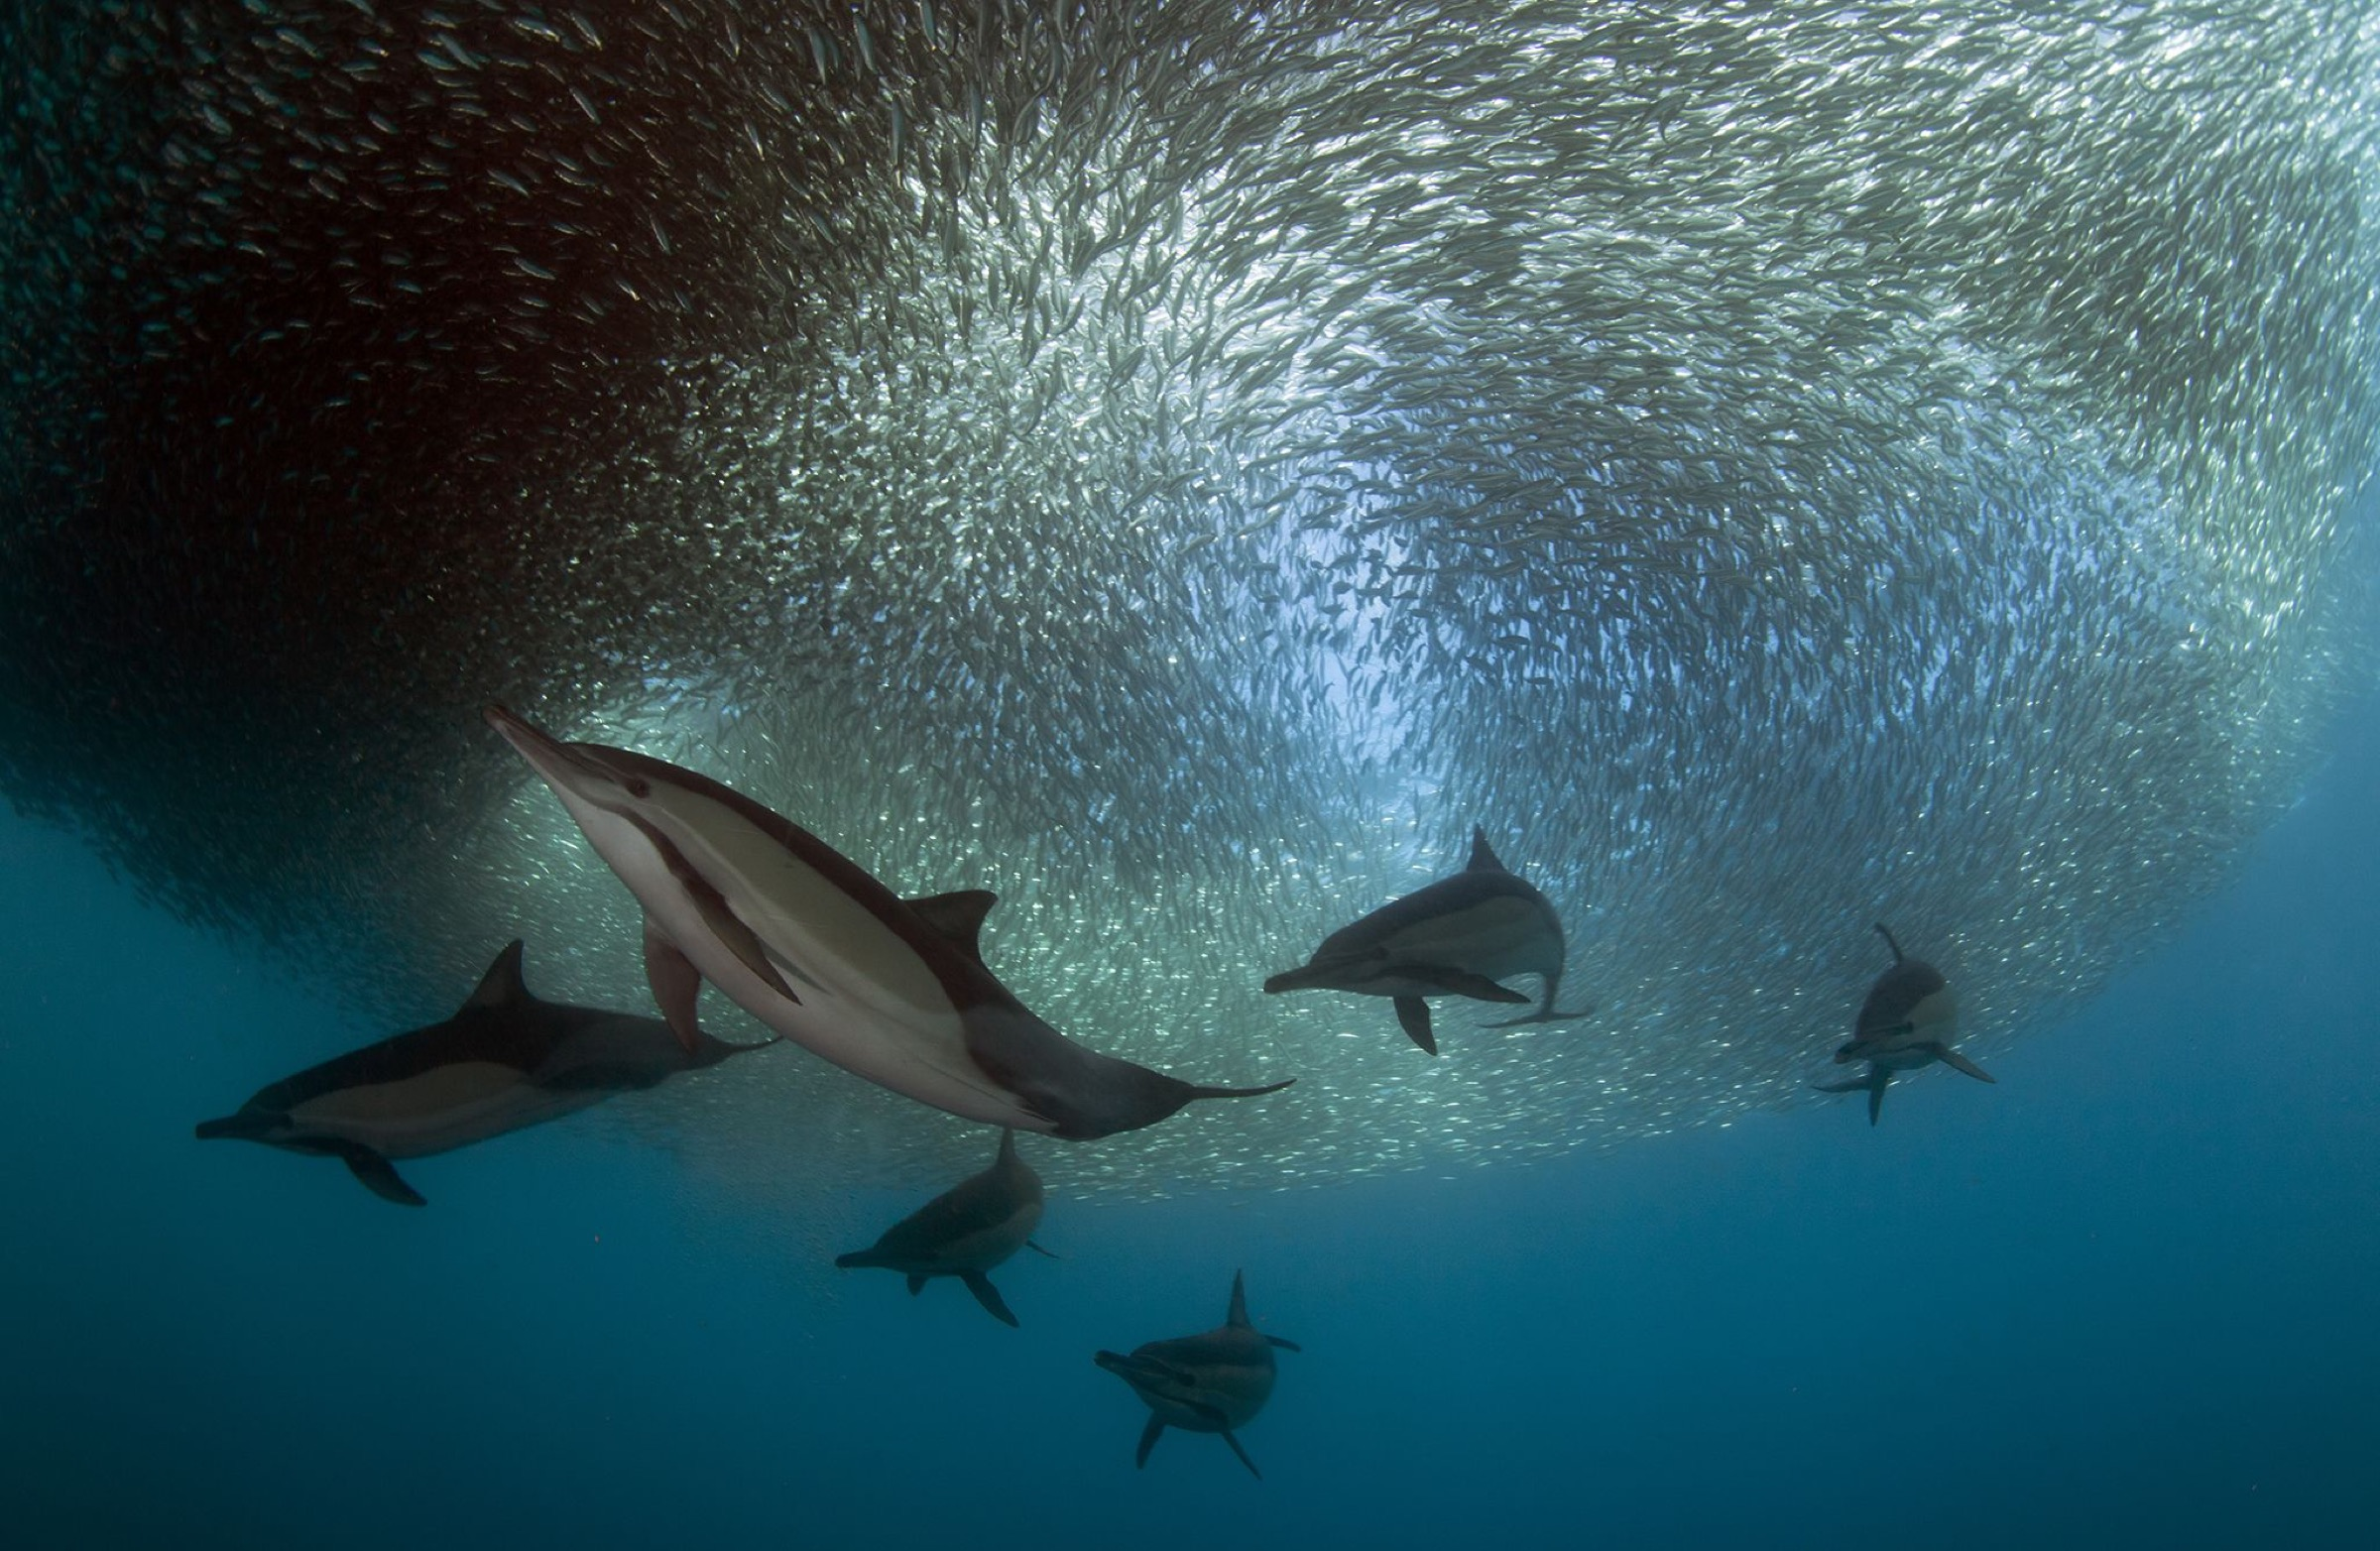
\includegraphics[scale = 0.1]{fish.jpg}			%path can be relative or absolute
    \caption{Shoal of Fish}
	\label{fig:T6Fish}			%so you can reference to the figure elsewhere using \ref{}
\end{figure}

Each fish can be represented by an agent with its own values. In a time-limited environment facing imminent danger, this species of fish will collectively organise, through the virtue of maximising their self-utility, which could be avoiding predation and surviving.\\

For example, by organising in this manner, each fish can observe a specific area and take action should there be a thread of predation. However, should these fish observe other fish acting in the same manner, in the belief that others will also try to avoid predation, these fish will mimic or replicate their actions to also evade predation. \\

Some use of 'Groupthink-informed decision-making' can minimise the cost of communication, dispute resolution and the computational cost of decision-making. 

\subsubsection{Dangers of Groupthink}

Unfortunately, groupthink can lead to irrational decision-making which can significantly reduce the collective utility. The assumption that each agent is rational and aims to maximise their self-utility may not be true and therefore mimicking others' behaviour can lead to some form of cascading alignment where overtime, mimicking others' behaviour will lead to a significant reduction in self and collective utility. \\

Additionally, extensive groupthink can erode away benefits gained from an efficient democratic system as described by the principles of 'democracy by design' which would tarnish the effectiveness of the democratic election process.

\subsection{Collective Intelligence informed Groupthink}

Using these ideas, team 6 proposes the system of 'Collective Intelligence informed GroupThink'.  This decision-making process aims to overcome the following issues:

\begin{enumerate}
  \item Provide a balance between \textbf{populism} and \textbf{expertise}
  \item\textbf{Maximise self-utility} whilst sustainably using common pool resources, hence avoiding the \textbf{tragedy of commons}
  \item Account for \textbf{power-grabbing} agents to avoid the formation of self-interested \textbf{oligarchies}
  \item Allow freedom of choice and enrich agent decision-making
\end{enumerate}

Considering the 8 foundational principles of democracy by design (DbyD), this system could improve the democratic process in place through the following principles: \cite{Jpitt}
    \begin{enumerate}
        \item[\textbf{P2}] Democracy is not an end-state, nor the default
        \item[\textbf{P3}]Seamless transition of power
        \item[\textbf{P5}] Visibility,. inclusivity, transparency, and accountability
        \item[\textbf{P6}] Inter-dependence of diversity 
        \item[\textbf{P7}] Education in the recognition of prosocial benefits
        \item[\textbf{P8}] Procedural Evaluation
    \end{enumerate}
\subsubsection{Assumptions}
This system assumes the following:

\begin{enumerate}
    \item Uncommon knowledge is distributed amongst agents
    \item There is significant diversity among agents
    \item Most agents are rational such that they aim for self-preservation and maximising self-utility.
\end{enumerate}\\

\subsubsection{Formalisation}
$SC_i$ is used to calculate how effectively each agent is able to maximise their self-utility at the cost of common pool resources, other agents and the resources available to them. 


$$SC_i = \sum_{j}^{n} (AgentState_j) + \alpha G_i + \beta B_i + \gamma L_i - e^{-\lambda T_i}$$
$$ AgentState = 
\begin{bmatrix}
HP\\
A\\
D \\
S \\
\end{bmatrix}
$$

Should there be an agent which can maximise this, it shows a level of expertise. As a result, should this be high enough, the agent will temporarily give them preferential voting in elections, similar to Groupthink. Meanwhile, once this expertise is identified, this agent can observe their actions as a learning mechanism to see how they can also achieve this. This calculation is procedurally evaluated at the start of each round.

\subsubsection{Limitations}

Given limited diversity, this system of decision-making is susceptible to populism voting and eventually very limited learning and progression. This became very clear in initial testing when only 2 agent types were used and eventually, there was usually convergence to single leadership. Additionally, when using random agents, this system becomes unreliable, however, it remained safe from the dangers of Groupthink mentioned above.\\

Therefore, this system requires significant diversity in agents to provide distributed diversity of knowledge as well as the common knowledge to act on this. 


\section{Experiments and Evaluation}

Experiments were conducted to evaluate our agent relative to a completely random agent. Due to problems with the game infrastructure, a completely fair comparison was not possible. Experiments showed that random agents were allocated items, but team's implementations of agents were not (when tested in isolation). Therefore any out-performance of the random agent was much more significant than the numbers suggest.\\

20 trials of three separate experiments were conducted:

\begin{enumerate}
    \item 100 random agents
    \item 100 team 6 agents, coded as per this report
    \item 100 team 6 agents with random parameter initialisations
\end{enumerate}

Experiment 3 involved randomly generating the initial parameters for the agents. This included all thresholds in fight / loot proposals and decisions, and all parts of leadership manifestos. The outcome of the experiments is summarised in table \ref{tab:T6Experiments}.

\begin{table}[h]
    \centering
    \begin{tabular}{||c|c|c||}
        \hline
       Agents & Mean Rounds & S.D\\
       \hline \hline
       Random & 27.8 & 0.40\\
       \hline
       Team 6 Random & 30.8 & 0.81\\
       \hline
       Team 6 Standard & 31.5 & 0.67\\
       \hline
    \end{tabular}
    \caption{Team 6 Experiments}
    \label{tab:T6Experiments}
\end{table}

The results clearly show that the Team 6 agent, configured with initial parameters as per this report, performed better than the random agent, even though the random agents were given items and the Team 6 agents weren't. The various strategies discussed in this report, including using Social Capital and Distributive Justice, have combined to produce an agent that is more likely to escape the pit than an agent that does not use some form of logic or informed strategy.\\

It is regretful that the game infrastructure and other team's agents were not in a state to run a full test game. The agent was designed to play the game alongside agents using different strategies, and to learn from them where possible. The lack of items also meant that the trading strategy outlined, whilst coded, wasn't utilised in the experiments mentioned.

\section{Future Improvements}

One big improvement that, given more time, would take the agent to a whole new level, is to utilise communication between agents. The Social Capital values discussed were designed to be communicated (hence the word `Social') between agents, with cliques and oligarchies potentially forming. It would be interesting to see the social networks that form, and what impact they have on the outcome for both the individual and the collective.\\

Another improvement would be to allow all fixed constants to be variable. Primarily for time and simplicity reasons, many values such as weights in calculations are fixed. However, allowing these to change during the game, as agents learn which characteristics are more important, would allow for more diversity even amongst a group of Team 6 agents.
